\documentclass[a4paper,oneside,onecolumn,article,draft]{memoir}
\counterwithout{section}{chapter}

\usepackage[T1]{fontenc}
\usepackage[utf8]{inputenc}
\usepackage{kpfonts}

\usepackage{textgreek}

\usepackage[final]{graphicx}

%% remove colorlinks option when ready for print
\usepackage[final,hyperindex,hyperfootnotes,bookmarksnumbered,colorlinks]{hyperref}

\usepackage{amsmath}

\newsubfloat{figure} % allow subfigures

\usepackage[textsize=footnotesize]{todonotes}
%% new command for box about missing references
\newcommand{\addref}[1]{\todo[color=red!40,size=\tiny]{Add reference: #1}}

\usepackage{tikz}

\usepackage[sectionbib,round,comma]{natbib}
\bibliographystyle{agu}

\usepackage{siunitx}
\DeclareSIUnit{\bp}{bp} % base pairs
\newcommand{\pcent}[1]{\SI{#1}{\percent}}
\newcommand{\dc}[1]{\SI{#1}{\degreeCelsius}}

\newcommand{\captionIntro}[2]{\caption[#1]{\textbf{#1.} #2}}

%% Just like we have cite and citep to cite in text and between parentheses,
%% have the same for fref, tref, etc...
\newcommand{\frefp}[1]{(\fref{#1})}
\newcommand{\Srefp}[1]{(\Sref{#1})}

\newcommand{\species}[1]{\textit{#1}}
\newcommand{\command}[1]{\texttt{#1}}

%% NCBI Style Guide, Chapter 5 "Style Points and Conventions", recommends
%% italic for gene names (except in long list of genes), and roman for
%% protein names.
\newcommand{\gene}[1]{\textit{#1}}
\newcommand{\protein}[1]{#1}

\newcommand{\kon}{$k_{on}$}
\newcommand{\koff}{$k_{off}$}
\newcommand{\halflife}[1][]{$t_{1/2}$#1}

\newcommand{\G}[1]{G$_#1$}  % for G0, G1, and G2 phases


\author{David Miguel Susano Pinto \and Kevin F. Sullivan \and Andrew Flaus}
\title{Application of FRAP to histones in human cell nuclei}

\begin{document}

  \maketitle

  \begin{abstract}
    Nucleosomes enable the stable compaction of almost all eukaryotic
    genomes but also require dynamic properties to enable access to
    the packaged DNA sequences.  The stability of core histones within the
    nucleosome should be reflected in their capability for dynamic exchange by
    Fluorescence Recovery After Photobleaching (FRAP).  To assay the
    effect of histone SWI/SNF INdependence (SIN)
    mutants known to destabilise nucleosomes
    \textit{in vitro} and in \species{S. cerevisiae}, we sought to
    apply FRAP to chromatin in mammalian cell lines.  This uncovered a
    number of challenges resulting from cell motility, nuclear movement
    within the cell, and chromatin motion within the nucleus with the
    long time frames required for FRAP of histones.  We were able to
    compensate for the former difficulties by a combination of cell
    biological and computational techniques, but we were unable to
    establish an appropriate approach to compensate for motion of the immobile
    binding sites required for standard FRAP analysis.
    Visualisation using photoactivated tagged histones in inverse FRAP
    demonstrated the extent of this chromatin motion
    and a further complexity arising from complex
    non-homogenous channelling tagged histone
    during diffusion.  This reveals the
    limitations of FRAP over extremely long time scales, and suggests
    that this technique is unsuitable for quantitative measurement of
    histone dynamics in the mammalian nucleus.
  \end{abstract}

  \section{Introduction}

  \subsection{Histones contribute to nucleosome dynamics}

    The chromatin packaging of eukaryote genomes performs the
    functions of compacting very large lengths of DNA into the
    microscopic cell nucleus, facilitating chromosomal movements
    during cell division, and providing a substrate for molecular
    mechanisms acting on the genome.

    The building block of eukaryotic chromatin structure is the
    nucleosome, comprising \SI{147}{\bp} of DNA wrapped around an
    octamer of two copies each of core histones
    H2A, H2B, H3, and H4 \citep{luger1997crystal}.
    Two H2A/H2B dimers flank a central H3/H4 tetramer.
    Nucleosome core particles are arranged
    in a linear chain separated by DNA linkers, and can be further
    compacted into higher order chromatin structures.

    Chromatin functions at both the molecular and cellular levels
    require the capability for dynamic rearrangement.  Chromatin
    structure can be modulated through nucleosomes by changing the
    arrangement of histones and DNA in a process known as remodelling
    \citep{flaus2011mechanisms}, or by altering histone chemical
    composition through post-translational modification
    \citep{bannister2011ptm-review}, or exchange of histone variants
    \citep{TalbertHenikoff2010}.

    A large amount of evidence has been accumulated about the static
    structure of the nucleosome at atomic resolution
    \citep{mcginty2014histone}, and about the arrangement of polymeric
    chromatin \citep{kuznetsova2016chromatin}.  However, the
    mechanisms for dynamic rearrangement of chromatin are much less
    well understood or integrated between the molecular and polymer
    levels \citep{andrews2011nucleosome}.

  \subsection{Nucleosome dynamics and histone SIN mutants}

    The archetype of ATP-dependent nucleosome remodelling enzymes is
    the SWI/SNF complex, which was identified in screens for mating
    type SWItching \citep{SWI-mutants} and Sucrose Non Fermentation
    \citep{SNF-mutants-original-discovery, SNF-mutants2} in
    \species{Saccharomyces cerevisiae}.

    Mutations were subsequently identified to compensate for the
    loss of the SWI/SNF complex that are collectively known as SIN
    mutations because they provide SWI/SNF INdependence
    \citep{kruger1995amino}.  A subset of SIN mutants are single
    amino-acid changes in core histones H3 and H4, providing a direct
    link between SWI/SNF and chromatin.  This also suggests the
    mutated residues in the histone proteins influence the same
    pathways for nucleosome dynamics leveraged
    by the remodelling enzyme and that
    these residues are significant for nucleosome stability.

    The prediction that the stability of SIN mutant containing
    nucleosomes would be affected in chromatin has been tested \textit{in vitro}
    where it was observed that SIN mutant nucleosomes display higher
    thermally driven nucleosome sliding mobility \citep{flaus2004sin}
    and that the mutated residues affect histone-DNA contacts in
    crystal structures \citep{muthurajan2004crystal}.

    However, the effect of histone protein SIN mutants
    in the more complex \textit{in vivo} chromatin environment
    of mammalian cells has not been demonstrated.
    Validating the functional significance of these residues
    is important for explaining the high conservation of
    histone protein sequences in eukaryotes.

  \subsection{Fluorescence Recovery After Photobleaching}

    Fluorescence Recovery After Photobleaching (FRAP) is an optical technique
    that can be used to report the dynamics of fluorescently
    tagged molecules within live cells.
    Tagged molecules inside a small region are irreversibly photobleached by
    a high power focused laser beam and the recovery rate of fluorescence
    in the bleached area is measured. The recovery rate is interpreted
    as unbleached fluorescing molecules from outside the region
    at the time of photobleaching diffuse into the bleached area.
    It is assumed that this fluorescence recovery
    reflects natural protein movement.

    A simple chemical equilibrium underlies the model for FRAP for a
    molecule with a single binding reaction:

    \begin{displaymath}
      F + S \overset{k_{on}}{\underset{k_{off}}{\rightleftharpoons}} FS
    \end{displaymath}

    where $F$ represents freely diffusing proteins,
    $S$ represents immobile vacant binding sites,
    and $FS$ is the complex between the two when the
    proteins are bound to the sites.
    The value of \Kon{} and \Koff{},
    are estimated from the rate at which photobleached $F$
    is replaced in the $FS$ complex.
    However, to such simple reaction is added complexity once
    diffusion and space is considered.

    Ongoing development of FRAP has led to increasingly complex models
    that are both more precise and accurate than simple
    inverse exponential decay \citep{mcnally-frap-2010}.
    Despite their sophistication, FRAP require assumptions
    that are difficult to maintain over long experimental observation times.
    Firstly, equilibrium must be maintained throughout the entire experiment
    so that both \Kon{} and \Koff{} remain constant.
    This also requires that concentrations of both $F$ and $S$ remain constant.
    Secondly, distribution of the fluorescently tagged molecules
    must mimic the endogenous protein.
    And finally, the binding sites must be part of a large,
    relatively immobile complex
    on the time and length scale of the recovery.
    In addition, different FRAP models will have additional constraints
    based on the multiple assumptions involved on the design of a
    model \citep{mcnally-frap-2010}.

  \subsection{FRAP measurements of histones}

    FRAP has been extensively used to obtain qualitative and
    quantitative insight into the kinetic properties of chromatin bound
    proteins \citep{phair2000high, essers2005nuclear, agresti2005gr}.
    These rely on the established assumption that chromatin is
    relatively immobile in the interphase nucleus
    \citep{abney1997chromatin} since the factors show recovery
    on the scale of seconds to minutes.
    H2B--GFP \citep{KevinH2BGFP} has become
    the standard reference for immobile fraction in these
    FRAP experiments \citep{dey2000bromodomain, kuipers2011highly,
    jullien2016chromatibody}.

    However, the dynamics of the core histones themselves
    was measured by FRAP in a seminal
    and widely cited study by \citet{KimuraCook}. Multiple H2B
    populations were delineated with distinctive exchange rates.  Some
    \pcent{3} of H2B had a rapid recovery within minutes, \pcent{40}
    had slow recovery with a \halflife[] of \SI{130}{\minute},
    and over \pcent{50} of H2B molecules had a
    very slow recovery with \halflife[] of
    over 8 hours that was considered to be effectively immobile.

    In contrast to H2B which is a histone dimer component, the tetramer
    histones H3 and H4 were found to have even slower mobility.  There
    were no rapid populations, with only slow and very slow populations
    of \SIrange{16}{22}{\percent} and \SIrange{62}{68}{\percent} being
    identified.

    In combination with additional heterokaryon data, Kimura and Cook
    interpreted the rapid, slow, and very slow exchanging H2B
    populations as correlating with transcription units, euchromatin,
    and heterochromatin respectively.  They assigned over \pcent{80}
    of H3 and H4 as immobile, whereas the remaining
    \SI{\approx 20}{\percent} was suggested to be mobilised by
    remodelling.  This latter small but significant
    slowly exchanging fraction of histones
    provides an opportunity to observe the dynamics of
    tetramer histones such as SIN point mutants in live mammalian cells.

    %% Their mobile fraction was odd.  The claim is that it represents
    %% the freely moving histones, but the text says that it was the
    %% recovery before the first post-bleach image could be acquired.
    %% This sounds like they assumed complete photobleaching.
    %% However, it can be that this is actually the unbleached
    %% fraction or some other background.

  \subsection{Aims and objectives}

    In order to test the implications for nucleosome structure and function
    of metazoan H4~R45H that exhibited the highest increase
    in nucleosome mobility \textit{in vitro} amongst
    the histone SIN mutants \citep{flaus2004sin},
    we set out to determine its exchange characteristics by FRAP.

    In attempting to achieve quantitative measurements
    we addressed multiple technical challenges associated with
    measuring subtle kinetic alterations of nucleosome dynamics
    over long time periods in live cells.
    This allowed us to define the limitations of FRAP for observing molecules
    such as core histones with extremely slow exchange rates.

  \section{Materials preparation}

  \subsection{Plasmid construction}
    Plasmids for the canonical histones H2B, H3, and H4,
    respectively pBOS--H2B--GFP \citep{KevinH2BGFP},
    pBOS--H3--EYFP.MC--N1, and pBOS--H4--ECFP.M--N1,
    were provided by Prof. Kevin Sullivan from National University of Ireland,
    Galway (NUIG). DNA sequencing identified the H3 plasmid as the \gene{HIST1H3B} gene,
    encoding H3.1 from histone cluster 1; the H4 plasmid as either
    \gene{HIST1H4J} or \gene{HIST1H4K};
    and the H2B plasmid similar to \gene{HIST1H2BJ} but with missense mutations D25G and V118I.
    Plasmid pPAGFP--N1 and mCherry--\textalpha--tubulin were provided by Chelly van Vuuren
    and the HeLa cDNA library was a kind gift of Nadine Quinn \citep{NadineThesis}.
    Plasmid pMH3.2--614 including a mouse replication dependent histone~H3
    gene with upstream and downstream regulatory elements \citep{pMH3-plasmid},
    was provided by Prof. Kevin Sullivan.

    \paragraph{H2B--EGFP}
      The D25G and V118I mutations in pBOS--H2B--GFP were corrected by PCR mutagenesis
      using primers AFG114 and AFG115, and AFG112 and AFG113 respectively.
      The resulting product is H2B--EGFP, equivalent to the HIST1H2BJ gene product fusion.

    \paragraph{H4--ECFP R45H}
      The R45H mutation was applied to the pBOS--H4--ECFP.M--N1 by
      PCR mutagenesis using the primers AFG124 and AFG125. The codon
      \texttt{CAC} was selected for the histidine amino acid due to its
      higher codon usage in the human genome\citep{codon_usage}.

    \paragraph{H2A--EGFP}
      Plasmid pBOS--H2B--GFP was digested with KpnI and BamHI
      and the band corresponding to the linearised vector without the H2B sequence
      was purified by gel extraction. The \gene{HIST1H2AB} sequence was amplified
      from HeLa genomic DNA with primers AFG116 and AFG118 and ligated into the vector.
      This coding sequence is equivalent to the H2A used in the previous
      \textit{in vitro} studies to be compared \citep{flaus2004sin}.
      HIST1H2AE has the same gene product but a lower codon adaptation index
      and more complex predicted 5' mRNA secondary structures.

    \paragraph{H2AX--EGFP and S139 mutants}
      Cloning of H2AX was similar to \gene{HIST1H2AB} but used primers AFG130 and AFG131.
      Mutations to H2AX S139, an important site that is phosphorylated during
      DNA damage response, was performed at the same time of gene amplification
      since its location is close to the sequence 3' end. Primers AFG132, AFG133, and AFG134,
      were used with AFG130 to introduce mutations S139A, S139D, and S139E respectively.
      The mutation to alanine blocks, while mutation to aspartic and glutamic acid
      mimic phosphorylation. This strategy introduced an accidental frameshift mutation
      near the stop codon which was fixed by PCR mutagenesis using primers AFG400
      and AFG401.

    \paragraph{H2A.Z--EGFP}
      The H2A.Z sequence was amplified from an HeLa cDNA library
      using primers AFG121 and AFG122
      due to the existence of introns in the \gene{H2AFZ} gene.
      Purification of the amplicon and ligation to the linearised pBOS--EGFP vector
      was identical to the preparation of the H2A--GFP plasmid.

    \paragraph{H4--EYFP}
      The plasmids pBOS--H3--EYFP.MC--N1 and pBOS--H4--ECFP.M--N1 were
      digested with the restriction enzymes BamHI and NotI. After agarose
      gel electrophoresis, the EYFP insert and pBOS--H4 vector were purified
      by gel extraction. The two DNA fragments were ligated to construct
      pBOS-H4-EYFP. The same strategy was used to construct the EYFP tagged
      H4~R45H mutant.

    \paragraph{H3--EYFP T45A and T45E}
      Mutations to H3 T45 were inserted into the pBOS--H3--EYFP.MC--N1 by
      PCR mutagenesis. The primers AFG151 and AFG152 were used for the
      T45E mutation, and AFG153 and AFG154 for T45A.

    \paragraph{H2B and H3 PAGFP}
      The PAGFP insert was prepared from pPAGFP--N1 by PCR using the
      primers AFG478 and AFG479, the amplicon purified by agarose gel
      extraction, digested with NotI and BamHI, and finally cleaned by
      PCR purification.
      Both pBOS--H2B--GFP and pBOS--H3--EYFP.MC--N1 plasmids were also
      digested with NotI and BamHI to excise their tags, and the vectors
      purified by agarose gel extraction. The insert was finally ligated
      into the two vectors for pBOS--H2B--PAGFP and pBOS--H3--PAGFP.
      This strategy introduces a Proline to Arginine mutation in the
      linker for the H2B plasmid.
      %% This mutation in the H2B linker (DPPVAT to DPRVAT) was on purpose.
      %% We could have easily avoid it but would cost us one extra primer
      %% and it shouldn't be making a difference.

    \paragraph{pMH2B--GFP and pMH3--EYFP}
      %% I'm actually not sure if Kevin gave me the pMH3.2--614 or the
      %% pCA-TAG plasmid. I did not have any plasmid map or sequence, only
      %% the very small Figure 5 of his paper PMID:9024683
      %% I couldn't even use any standard sequencing primer and by the time
      %% we cloned our genes there, we had already decided to kill the project
      %% so we never got to actually try these in human cells.
      Insertion of the H2B--GFP and H3--EYFP coding sequences into the
      pMH3.2--614 plasmid was performed by PCR amplification, bluent-end
      ligation of both vector and inserts due to the absence of restriction
      sites. pMH3.2--614 was amplified with primers AFG417 and AGF418 which
      create a linear sequence that only ignore the H3.2 coding sequence.
      The H2B--GFP coding sequence was generated with primers AFG419 and AFG420.
      Primers for the insert were phosphorylated by T4~PNK prior to the PCR
      since T4~PNK is more efficient on single stranded DNA. pM vector and
      H2B--GFP insert were purified by agarose gel extraction and ligated.
      Strategy for H3--EYFP was equivalent but using primers AFG424 and AFG420.

  \subsection{Cell lines}

    Transfection was always performed by lipofection~\Srefp{methods:lipofection},
    both for transient and stable cell lines. For creation of stable cell lines,
    cells were trypsinized and split 1:20 on \SI{10}{\cm} dishes 24~hours after transfection.
    After another 24 hours, Blasticidin-S was added to the medium for
    a final concentration of \SI{3}{\ug\per\ml} as found by performing a
    Blasticidin-S kill-curve \Srefp{sec:methods:kill-curve}.
    Cell growth was followed and medium replaced when appropriate.
    As cell colonies started to be visible by the naked eye, approximately
    3~weeks after plating, these were screened by fluorescence microscopy.
    Positive colonies were aspirated and moved into 24-well plates with
    \SI{1}{\ml} disposable pipette tips, and the thinnest extremity removed.

    \begin{figure}
      \centering
      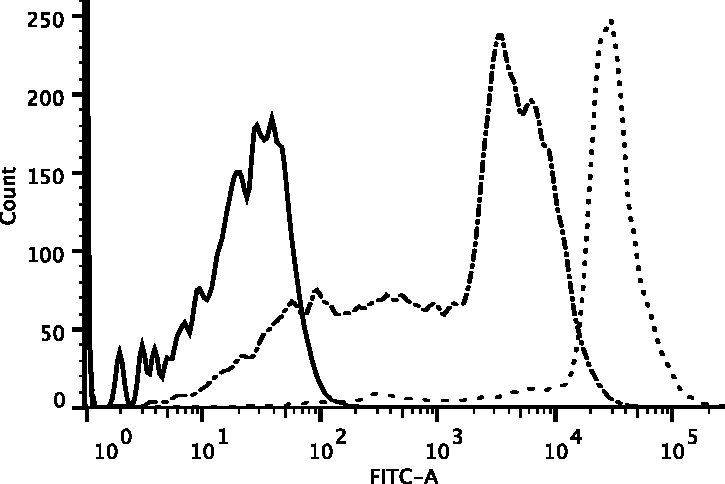
\includegraphics[width=\textwidth]{figs/facs-stable-cell-lines.pdf}
      \captionIntro{FACS sorting of mixed populations}
        {
          The multiple populations with differing intensity values were
          sorted by FACS. The full line represents the intensity profile
          of HeLa wild type cells; the dash-dot line, a mixed population
          of HeLa cells expressing H2B--EGFP; and the dotted line, the
          sorted population.
        }
      \label{fig:methods:facs}
    \end{figure}

    Populations with mixed levels of fluorescent intensity were frequently
    obtained while preparing stable cell lines. In such cases, cells with
    similar intensity of their corresponding fluorophore were FACS
    sorted \frefp{fig:methods:facs}.

    The following stable lines were prepared:

    \begin{itemize}
      \item HeLa H2B--EGFP
      \item HeLa H2B--EGFP D25G V118I
      \item HeLa H3--EYFP
      \item HeLa H3--EYFP T45A
      \item HeLa H3--EYFP T45E
      \item HeLa H4--EYFP
      \item HeLa H4--EYFP R45H
    \end{itemize}

  \subsection{Microscopy}

    Both stable and transiently cell lines were used in imaging as described.
    Transfection was performed 48~hours before imaging for transiently
    expressing cells.

    Confocal microscopy was performed with a Zeiss LSM510 Meta microscope
    using glass bottom LabTek II chambers. Wide-field fluorescence microscopy
    was performed with an Applied Precision DeltaVision Core system
    using \SI{35}{\mm} glass bottom MatTek dishes.

    In both cases, imaging was performed within an acrylic environmental
    chamber that fully enclosed the stage plate and microscope objectives.
    Temperature and CO$_2$ levels were maintained via separate units connected
    to the environmental chamber.

  \subsection{Computational analysis}

    Software used for image analysis and visualization was described in
    \Sref{sec:methods:software}. Original source code written in \textsc{Matlab} for a previously
    reported circle FRAP model \citep{mueller2008evidence} was kindly offered
    to us under the GNU General Public License (GPL) version~3 by the
    original authors. A port of this code for the GNU Octave language was
    prepared and made available under the same license.

  \section{Results}

  \subsection{FRAP analysis in Octave}

    In order to estimate binding constants from FRAP data, we ported
    \textsc{Matlab} code for circle FRAP \citep{mueller2008evidence} to GNU Octave.

    Functions for nonlinear regression were required for the model
    fitting and were replaced by \texttt{leasqr}
    from Octave-Forge's optim package. This function performs the
    Levenberg--Marquardt nonlinear least squares algorithm which is the
    same as the documented method for \texttt{nlinfit}.
    Several sample images were analyzed
    by the Octave port and the fitted values were found to be equal to
    the values reported by the authors using the original code (data not shown).
    Functions for graphical user interaction were mainly required
    for manual selection of Regions Of Interest (ROIs) and options.
    Selection of ROIs was replaced by automatic identifications
    and parameter input was made command-line based for batch processing.

    \subsubsection{ROI selection}

      Bleach spot, nucleus region, and background region ROIs are required
      for the circle FRAP model. The bleach spot measures intensity recovery
      and also models the photobleach profile since it takes into account
      a non-uniform spatial distribution of the bleached spot. The nucleus
      region defines the finite sized nucleus and takes into account
      the fluorescence loss during the photobleaching,
      while a small region outside the nucleus is used for background correction.

      Cells expressing GFP tagged histone proteins have well defined nuclei.
      The large amount of histone protein and specificity for nuclear chromatin
      produces a strong and clear signal for the nuclei contrasted on a dark background (\fref{fig:kill-frap:roi}).

      \begin{figure}
        \centering
        \subbottom[pre-bleach]{
          \includegraphics[width=0.45\textwidth]
          {results/roi-prebleach.png}
          \label{fig:kill-frap:prebleach}
        }
        \hfill
        \subbottom[post-bleach]{
          \includegraphics[width=0.45\textwidth]
          {results/roi-postbleach.png}
          \label{fig:kill-frap:postbleach}
        }
        \subbottom[pre-bleach $-$ post-bleach]{
          \includegraphics[width=0.45\textwidth]
          {results/roi-subtracted.png}
          \label{fig:kill-frap:subtracted}
        }
        \hfill
        \subbottom[Identified ROIs]{
          \includegraphics[width=0.45\textwidth]
          {results/roi-selected.png}
          \label{fig:kill-frap:selected}
        }
        \captionIntro{Automatic selection of ROIs for FRAP}
          {
            HeLa stable cell line expressing the H4~R45H mutant tagged with YFP,
            are imaged every \SI{30}{\ms} in a confocal microscope. A circular
            shape is used for photobleaching after 100~frames.
            \subcaptionref{fig:kill-frap:prebleach} averaging of 50~pre-bleach
            images removes most of the noise, allowing for a better refined
            ROI;
            \subcaptionref{fig:kill-frap:postbleach} average of
            5 post-bleach images;
            \subcaptionref{fig:kill-frap:subtracted} subtraction of the
            post-bleach to the pre-bleach image, gives a clear indication
            of the bleach spot, as well as faint signal for the nuclear
            region due to unintentional photobleaching;
            \subcaptionref{fig:kill-frap:prebleach} perimeter of the
            automatically identified ROIs superimposed on the pre-bleach
            image: cell nuclei, bleach spot, and background region.
          }
        \label{fig:kill-frap:roi}
      \end{figure}

      Subtraction of the post-bleach (\fref{fig:kill-frap:postbleach}) from
      the pre-bleach (\fref{fig:kill-frap:prebleach}) images displays
      a clear circular shape corresponding to the bleach spot (\fref{fig:kill-frap:subtracted}).
      The centre for this spot was identified by finding the maximum of the convolution matrix
      between the subtracted image and a disk kernel.
      To reduce signal-to-noise ratios, multiple pre and post-bleach images of the cell
      were averaged before image operations.
      While the bleach spot is the most visible feature, there is a faint nuclear region signal
      caused by background photobleaching during image collection.

      An approximate border for cell nuclei could be readily defined using Otsu's method for image threshold.
      As with the identification of bleach spots, multiple pre-bleach images
      were averaged before threshold definition for a more accurate cell border (\fref{fig:kill-frap:selected}).
      Since multiple nuclei often appeared in a single image, the coordinates for the bleach spot
      were used as reference to select the correct nucleus.
      The background region was identified by finding the minimum of the convolution matrix
      between the averaged pre-bleach images and a small square of black intensity values.

    \subsubsection{Batch processing}

      \begin{sidewaysfigure}
        \includegraphics[width=\textwidth]{results/frapinator.png}
        \captionIntro{Frapinator visual log files for batch processing}
          {
            Each FRAP experiment generates a log file with 6 different plots
            displaying the analysed values and the fitting to different models.
            In conjunction with the images in \fref{fig:kill-frap:roi} this
            provides a quick overview of the entire analysis process.
            The top left plot displays the raw intensity
            for the background, bleach spot, and nucleus intensity over the
            duration of the FRAP experiment. This is followed by the normalized
            intensity for the bleach spot which is actually used for the
            fitting. The top right displays the intensity
            profile for the bleach spot, and its fit to a radial profile
            model. The three bottom panels display the data fitted to three
            different models: pure diffusion which has no terms for binding
            constants; full model with a fixed diffusion rate; and full model
            with all the 3 terms.
          }
        \label{fig:kill-frap:frapinator}
      \end{sidewaysfigure}

      The automated identification of ROIs was turned into a stand-alone program, frapinator.
      This has the advanatge that the user can set command-line options without scripting.
      Representative images are saved with results and all intermediate analysis is logged for post-processing analysis.
      These include the automatically identified ROIs and
      plots of measured intensities, bleach spot profile, and fitting to different models \fref{fig:kill-frap:frapinator}.
      Frapinator is available for public download under the GPL \footnote{\url{https://github.com/github/octave-frap}}.

  \subsection{Tracking of cell nuclei}

    %% We could show this but it would only be to "encher chouricos"
%    \begin{figure}
%      \centering
%      \missingfigure{Our first FRAP experiment}
%      \captionIntro{Long time series of HeLa cells expressing H2B--EGFP.}
%                   {Cells were transfected with pBOS--H2B-EGFP and imaged for 8
%                    hours, with intervals of 20 minutes.}
%      \label{fig:kill-frap:cell-movement}
%    \end{figure}

    Histone proteins exhibit extremely slow kinetics of exchange
    requiring FRAP to be performed over several hours during which cell movement is
    a particular issue. % \fref{fig:kill-frap:cell-movement}.

    %% This needs some sentences describing the nature of effects of the movement,
    %% and a semi-emirical statement of the scale of the movement
    %% since this problem is the nub of the entire chapter.
    %% Need to justify the need for going to the trouble
    %% and define threshold for success (that couldn't be achieved!)

    The central requirement to accurately identify and quantitate the signal
    in the photobleached spot led us to pursue both cell biological approaches to
    minimise cell movement and and computational approaches to track imaged regions.

    \subsubsection{Contact inhibition at high cell density}

      Mammalian cells display contact inhibition,
      a cellular growth mechanism by which cells enter senescence and reduce motion
      when surrounded by other cells with no free space for movement.
      Although transformed cell lines lose this property,
      reduced space does place a restriction in the movement.
      %% Can you provide a semi-quantitative estimate of the cell density you mean?
      We attempted to use this effect to limit movement of cells
      by performing FRAP measurements with cells at higher confluence levels.
      We observed some decrease of movement for HeLa cells but not a complete immobilization.
      %% Can you provide a semi-quantitative estimate of the degree of reduction in movement?

      \begin{figure}
        %% We are only showing one cell rather than the whole field of
        %% of view because otherwise it's hard to notice the movement of
        %% individual cells. If we do display everything, we cell many
        %% nuclei that seem like their movement is smaller. If we do
        %% show it, we comment that we are unsure whether the movement
        %% is cellular or only nuclear.
        \centering
        \includegraphics[width=\textwidth]{results/confluent-hela.png}
        \captionIntro{Movement of confluent HeLa cells during FRAP experiment}
          {
            Cells reached confluence before the start of the
            experiment in an attempt to reduce motion. Instead, this caused
            cell nuclei to undergo heavy reshape as the cell apparently
            squeezes in between its neighbours. Half-nuclear FRAP performed in
            a confocal microscope over an interval of 8~hours. Top left panel
            is the pre-bleach image, while the others have a time-interval of
            21~minutes. Cells are a stable line derived from HeLa, expressing
            the H4~R45H mutant tagged with YFP.
          }
        \label{fig:kill-frap:confluent-hela}
      \end{figure}

      Tracking of the ROIs over time was still required \fref{fig:kill-frap:confluent-hela}.
      %% Isn't this out of order since CropReg section is below.
      %% Even if you did it in a different order, why not put the horse cells first.

    \subsubsection{Primary cell lines}

      Since HeLa cells have lost the ability to activate contact inhibition,
      we obtained an immortalised primary horse fibroblast cell line
      that displayed contact inhibition. Using this cell line we could
      maintain a layer of healthy cells covering a Petri dish for several days???
      after reaching confluence (data not shown).
      %% Cell growth was halted instead of becoming over-confluent ???what do you mean???
      %% Although obvious, it would be good to have some sort of image to justify the statement?

      However, primary cell line transfections have typically much lower efficiency rate and
      confluent cells have lower expression with each cell division.
      To balance transfection efficiency and expression we transfected cells at
      \SI{70}{\percent} confluence and imaged them after 3 days.

      Even after reaching confluence, we observed movement of transfected horse cells \fref{fig:kill-frap:confluent-horse}.
      %% Is there some sort of relative statement about the degree of reduction or residual movement?
      In addition, the observed movement was dramatically different in primary horse than in HeLa cells.
      Transfected horse cells displayed a helical motion about the vector of their movement
      whereas rotation of HeLa nuclei was mostly restricted to the $z$ axis.
      %% You need to define the coordinate system to talk about z axis!
      %% Do you mean vertical relative to the cell dish layer?

      \begin{figure}
        \centering
        \includegraphics[width=\textwidth]{results/confluent-horse.png}
        \captionIntro{Movement of confluent primary cells during FRAP experiment}
          {
            Primary horse fibrolasts display contact inhibition and halt growth
            once they reach confluence. However, this does not stop cell
            motion which can still be seen moving. In addition, when compared
            to the cancer cell line HeLa (\fref{fig:kill-frap:confluent-hela}),
            the horse fibroblasts frequently rotated around the $x$ and $y$
            axis. Circle FRAP was performed in a widefield microscope.
            Top left panel is the pre-bleach image, while the others have a
            time-interval of 15~minutes. Cells were transiently transfected
            and are expressing H2B type1-J tagged with EGFP.
          }
        \label{fig:kill-frap:confluent-horse}
      \end{figure}

    \subsubsection{Tracking of cell movement}

      As an alternative strategy, we implemented cell tracking
      in order to transform images into a common frame using
      consecutive image cropping and image registration.
      This approach was implemented as a program named CropReg.

      Nuclei of interest were tracked by template-based matching using normalized cross-correlation.
      Briefly, the nucleus to track was identified on the first frame and
      used as template against the image on the subsequent frame.
      For increased performance and robustness only the region surrounding the original position is used.
      %% Should you state approximately how large this region was?
      Sequentially applying this method created a stack of smaller images centred on the nuclei of interest.

      Achieving this functionality required implementing a ``coeff'' option
      for scaling in the \texttt{xcorr2} function in GNU Octave.
      This was contributed and released in version 1.2.0 of the Octave Forge signal package.
      %% TODO since there's more than one way to actually do the normalization,
      %% it might be a good idea to write down the actual math formula
      To correct for rotational movement around the $z$ axis,
      frames were aligned using rigid body geometric transformation using ImageJ plugin StackReg \citep{stackreg}.

      \begin{figure}
        \centering
        \includegraphics[width=\textwidth]{results/cropreg.png}
        %% imaging was done every 10 minutes, but we are skipping
        %% every other panel
        \captionIntro{Automatic tracking and alignment of moving cells}
          {
            Using CropReg, we successfully tracked individual cells during
            a time-series microscope experiment. The top left corner of each
            panel displays the tracked and aligned cell. Imaging was performed
            in a widefield microscope. Time interval between panels 20~minutes.
            Cells are a stable line derived from HeLa, expressing H3 tagged
            with YFP.
          }
        \label{fig:kill-frap:cropreg}
      \end{figure}

      Using this image processing approach we were able to track individual cell nuclei
      throughout an entire sequence of FRAP experiments \fref{fig:kill-frap:cropreg} provided
      that nuclei did not overlap.
      Although only a small minority of image sequences satisfied this requirement,
      it was possible to collect sufficient observations for FRAP calcultions.

  \subsection{Chromatin movement}

    While performing the FRAP experiments, we observed some movement
    within the cell nuclei. These could not be accounted for simple rotational
    movement around the $x$ or $y$ axis, and resembled more the movement
    of individual bodies within the nuclei.

    \subsubsection{Selection of \G1{} cells}
      %% There's no chemical equilibrium in S phase

      A possible cause of this chromatin movement comes from changes in
      the cell cycle phase. During the S~phase, the DNA is replicated,
      doubling the content of the chromatin.
      More importantly, this breaks
      a core assumption of FRAP, that the system remains in equilibrium
      during the entire experiment. This does not hold if the DNA, the
      binding sites for our model, duplicate in number.

      If the FRAP experiments can't be performed during S~phase and
      mitosis, we are limited to \G1{} and \G2{}. Considering
      the length of the HeLa cell cycle and the requirements to image
      for a time period of 8~hours, we are further limited to \G1{}.
      In addition, the FRAP experiment must be performed early in
      \G1{}~phase to avoid crossing over to the S~phase.

      %% The only reason this was required was because the LSM 510
      %% that we were using could not make Z stack and time lapse
      %% at the same time.
%      \begin{figure}
%        \centering
%        \missingfigure{Hela cells splitting}
%        \captionIntro{Picking cells at early G$_1$.}
%                     {We imaged cells that were entering mitosis and picked their
%                      daughter cells for the FRAP experiments. Because HeLa cells lift
%                      away from the dish during mitosis, opening the
%                      pinhole and set the Z-center in between the cell dividing plane
%                      and dish bottom was necessary. Ends up nothing being properly in focus but we
%                      can track things fine. Of course, some cells still floated away.}
%        %% TODO explicit parameters
%        \label{fig:kill-frap:picking-early-g1}
%      \end{figure}

      To do this, cells in mitosis were selected and tracked during 4~hours.
      After this time period, we used the daughter cells which we could be
      confident of being in early \G1{}.
      %% we also waited some 2 hours after mitosis since that's when cells
      %% unpack their chromosomes.

      During mitosis, HeLa cells form a sphere slightly above the plane of
      other cells, and keep a weak connection to the growth surface.
      Because of this, they easily detach, which is the basis for the
      mitotic shake-off method, and float away from the field of vision
      which requires a larger number
      of initial selected cells. In addition, to minimize any effect that
      may arise from imaging, it was done at minimal laser power and every
      30~minutes, just enough to allow manual tracking.
      Finally, since our system did not permit simultaneous Z-stack and time
      lapse imaging, and cells in mitosis are in a separate focal plane,
      imaging was performed with the pinhole sized to the max and focused
      in between the two planes. While this
      created very blurred images, it allowed to visualize all cells during
      the entire procedure.

      However, even after selecting cells in this cell cycle, movement within
      the bleach spot could still be observed.

    \subsubsection{Inverse FRAP}

      Due to the non-homogeneous nature of the chromatin, it was difficult
      to assess the total extent of the observed movement. To
      better visualize this, we performed inverse FRAP which allows us
      to track the movement of the bleach spot only.

      For this purpose, we replaced the EGFP tag in our H2B plasmid
      with photoactivatable GFP (PAGFP), a GFP derivative that requires
      activation by a specific wavelength to become fluorescent. This
      allows us to activate a specific spot of the nucleus and visualize
      its movement.

      Since PAGFP cannot be easily detected before photoactivation, cells
      were co-transfected with mCherry--\textalpha--tubulin which localises
      exclusively to the cytoplasm, giving an outline of the nuclear region
      \fref{fig:kill-frap:ifrap}.

      \begin{figure}
        \centering
        \subbottom[pre-activation]{
          \includegraphics[width=0.45\textwidth]
          {results/ifrap-pre.png}
          \label{fig:kill-frap:ifrap-pre}
        }
        \hfill
        \subbottom[post-activation]{
          \includegraphics[width=0.45\textwidth]
          {results/ifrap-post.png}
          \label{fig:kill-frap:ifrap-post}
        }
        \subbottom[activated spot over time]{
          \includegraphics[width=\textwidth]
          {results/ifrap.png}
          \label{fig:kill-frap:ifrap-timeframe}
        }
        \captionIntro{Inverse FRAP experiment showing chromatin movement}
          {
            HeLa cells co-transfected with mCherry--\textalpha--tubulin and
            H2B type1-J tagged with PAGFP.
            \subcaptionref{fig:kill-frap:ifrap-pre} The cell nucleus, target
            for photoactivation, can be easily identified as the ``empty''
            region via the mCherry channel on which would otherwise be an
            invisible feature on the GFP channel;
            \subcaptionref{fig:kill-frap:ifrap-post} spot after activation;
            \subcaptionref{fig:kill-frap:ifrap-timeframe} detail of the
            activated spot every 20~minutes. Rather than a gradual loss of
            fluorescence that maintains the circular shape, the activated spot
            kind of unfolds itself spreading the region of interest.
          }
        \label{fig:kill-frap:ifrap}
      \end{figure}

      Using this FRAP variant, the movement of chromatin was more noticeable.
      Rather than an homogeneous loss of fluorescence, the activated
      spot uncurled itself overtime with individual branches of
      localized PA-GFP appearing in the nuclei (\fref{fig:kill-frap:ifrap}).

  \section{Discussion}

    We wished to quantitatively determine the
    effect on human chromatin stability
    of SIN mutations in core histones H3 and H4 known
    to be destabilising \textit{in vitro} and to affect
    cell growth in \species{S. cerevisiae}.
    We set out to use a previously reported circle FRAP model
    which accounts for multiple factors in a typical
    FRAP modelling \citep{mcnally-frap-code}.

    However, FRAP recovery is incomplete even
    after 8~hours for core histones \citep{KimuraCook}.
    This led us to address a series of technical challenges in
    collecting valid quantitative recovery data over extended time periods.

% Cell movement

    The first problem faced was cell movement.
    This is an expected property of actively dividing cells.

    We attempted to reduce motion by taking advantage of
    the fact that many primary cells display contact inhibition of
    locomotion and proliferation when they reach high densities.
    This contact inhibition is a natural mechanism
    that controls cellular growth in
    multicellular organisms, and results in a stop to proliferation
    with formation of a monolayer of healthy cells in tissue culture.

    However, this approach has disadvantages including
    increased cell handling and reduces transfection efficiency,
    and means that stable cell lines based on
    immortalised cells cannot be used.
    The potential inability to compare results with published data for
    immortalised cell lines such as HeLa is also disadvantageous.

    Despite achieving a monolayer of healthy cells that
    could be maintained stably over 2 weeks,
    individual transfected primary horse fibroblasts still showed some movement
    despite exhibiting overall characteristics of contact inhibition.
    Furthermore, nuclei in these cells displayed a helical motion
    on the direction of cell movement \frefp{fig:kill-frap:confluent-horse}.

    The possibility of chemically inhibiting
    cells to reduce motion was considered
    since previous FRAP experiments with core
    histones were performed using multiple inhibitors
    of protein synthesis \citep{KimuraCook}. However, these studies revealed
    inhibitor-dependent variations in kinetics and the authors qualified
    their conclusions about the absolute accuracy
    of exchange parameters measured.

    To better address the problem of cell movement we
    instead developed a computational approach
    by writing a program for cell tracking by normalised
    cross-correlation template matching.
    Using automated analysis enabled us to process
    the large numbers of cell images
    required to provide statistically valid
    quantitative measurements of core histone exchange.

% Compositional changes

    The second challenge to measuring core histone exchage by FRAP is that
    a chemical equilibrium is required between freely diffusing proteins and
    formation of a complex. Although absolute equilibrium is unlikely
    in the dynamic cell environment undergoing
    complex transcriptional and translation responses,
    DNA replication involving polymerase passage
    and repackaging of the duplicated genome
    in S~phase will clearly unbalance any equilibrium.

    Chromosome compaction in mitosis also generates a chromatin environment
    that is distinct from interphase.
    This limits FRAP experiment to either \G1{} or \G2{} phases.
    The HeLa cell cycle has a typical \G1{} phase of 11.7~hours
    and a \G2{} phase of 3~hours \citep{HeLaCellCycle}
    so the extended time periods needed for FRAP of core histones requires
    starting FRAP early in \G1{} \frefp{fig:kill-frap:cell-cycle}.

    Post-mitotic chromosomes take approximately 2~hours
    to migrate within the nucleus
    and rebuild the interphase nuclear architecture during early \G1{}
    \citep{visualizationG1chromosomes,earlyg1position,RelativeChromosomePosition}.
    This defines the window for extended FRAP experiments
    from approximately 3 to 11 hours after mitosis
    in HeLa cells, although cells lines with even longer
    \G1{} phase are known \citep{PancreaticCells}.

    We wished to avoid the use of drugs for cell
    cycle arrest since this has been
    shown to influence FRAP results \citep{KimuraCook}.
    We also discounted serum starvation to move cells into the
    quiescent \G0{} phase since this could affect
    the relevance of measuring core histone
    exchange \citep{SerumStarvation}.

      \begin{figure}
        \centering
        %% based on original code from Robert Vollmert
        %% http://www.texample.net/tikz/examples/pie-chart/
        \newcommand{\slice}[4]{
          \pgfmathparse{0.5*#1+0.5*#2}
          \let\midangle\pgfmathresult

          % slice
          \draw[thick,fill=black!10] (0,0) -- (#1:1) arc (#1:#2:1) -- cycle;

          % outer label
          \node[label=\midangle:#4] at (\midangle:1) {};

          % inner label
          \pgfmathparse{min((#2-#1-10)/110*(-0.3),0)}
          \let\temp\pgfmathresult
          \pgfmathparse{max(\temp,-0.5) + 0.8}
          \let\innerpos\pgfmathresult
          \node at (\midangle:\innerpos) {#3};
        }
        \begin{tikzpicture}[scale=3]
          \newcounter{a}
          \newcounter{b}
          %% Total cell cycle is 24.5 hours, G1 is 11.7h, S is 8.8h,
          %% G2 is 3h, M is 1h. The problem is that the counters can't handle
          %% decimal places so we have a variable with the actual time for
          %% the text, and another one times 10 to calculate the angle.
          \foreach \p/\t/\l in {117/11.7/\G1, 9/0.9/M,
                                31/3.1/\G2, 88/8.8/S}
            {
              \setcounter{a}{\value{b}}
              \addtocounter{b}{\p}
              \slice{36*\thea/24.5} % we multiply by 36 instead of 360 because
                    {36*\theb/24.5} % the time is already times 10
                    {\l}{\t{} hours}
            }
        \end{tikzpicture}
        \captionIntro{HeLa cell cycle phases and timing}
          {
            Under optimal growth conditions the HeLa cell has a median
            doubling time of 24~hours, with \G1~and
            S~phases of 11.7 and 8.8 hours respectively \citep{HeLaCellCycle}.
          }
        \label{fig:kill-frap:cell-cycle}
      \end{figure}

    Instead, we developed a procedure to track cells manually during mitosis
    where visual identification of the cell cycle is possible.
    This allowed us to minimise interventions
    and effects on the cell normal growth
    while identifying individual cells exactly 3 hours after start of \G1{}.
    It has the added advantage of allowing time for maturation of GFP
    expressed during the establishment of interphase.
    The time interval between images during manual selection was increased and
    both resolution and laser intensity reduced
    to minimise phototoxicity or bleaching.
    This resulted in a set of selected early \G1{}
    cells suitable for FRAP experiments.

    The fluorescently tagged histone proteins are constitutively expressed
    under the control of an EF-1\textalpha{} promoter,
    so they lack the 3' regulatory features of the native histone genes.
    This regulation does not follow the normal
    expression program of a histone gene
    and hence could alter the distribution of the histone in chromatin.
    Constant expression of tagged histones by a strong constitutive promoter
    will enrich them in the \G1{} and early S~phase pools
    making subsequent incorporation in euchromatin more likely,
    relative to mid-late S~phase where heterochromatic sequences
    are replicated and packaged \citep{DNA-replication-timing}.

    A more realistic tagged histone expression profile can be achieved using
    flanking regulatory regions from native histone genes,
    as demonstrated for H3 and CENP--A \citep{pMH3-plasmid,Kevin-pCA-TAG}.
    Another potential solution is to insert GFP
    in-frame into the native gene locus by genome engineering,
    although the redundancy between the multiple canonical histone genes means
    that identifying the most appropriate isoform to target
    could introduce complexities.

    Protein synthesis inhibitors were used by \citet{KimuraCook}
    to address this issue,
    but this has the disadvantage of potentially affecting
    many other processes as discussed above.

      %% TODO: would be cool to create this figure
%      \begin{figure}
%        \centering
%        \missingfigure{a schematic of cell cycle, soluble pool}
%        \captionIntro{Distribution of tagged and endogenous histones during cell cycle}
%                     {
%                       This would be at least 3 different subplots. The first
%                       and the second are like the ones in Fig 7A of Kimura and
%                       Cook paper. The third one would show the ratio of each
%                       histone over time, i.e., 100\% tagged during all cell
%                       cell cycle and some endogenous during S phase. In this
%                       plots, also note where euchromatin and heterochromatin
%                       are replicated.
%                     }.
%        \label{fig:kill-frap:messy-histone-expression}
%      \end{figure}

% Movement of the reference

    The final challenge to measuring core histone
    exchange by FRAP that we identified
    was non-homogenous regional movement of chromatin itself.
    This undermines the assumption of FRAP analysis that binding sites
    remain immobile throughout the FRAP experiment.
    This assumption is required to interpret recovery
    as the rate of movement of freely diffusing unbleached molecules into the
    bleached area which allows the kinetic
    rates \Kon{} and \Koff{} to be estimated.
    If chromatin binding sites also move then the recovery curve becomes a
    much more complex function of both binding site movement and free diffusion.

    Chromatin movement is recognisable both
    by changes in the intra-nuclear features of the fluorescent chromatin
    and by changes in the circular bleach spot.
    Although some of these effects are subtle when observed by photobleaching,
    the circle photoactivation by inverse FRAP demonstrates
    clear non-homogenous reshaping of chromatin.
    Equivalent chromatin movement has also been reported
    for H4--PAGFP in strip photoactivation \cite{H4PAGFP-chromatin-movement}.

    The movements we observed were in the
    range of \SI{4}{\um}, which is double the size of the bleach spot,
    and exhibited complicated shapes reminiscent of channelling.
    This is consistent with chromosome distribution in nuclei that is
    territorial on the scale of \SI{5}{\um} \citep{sun2000size}
    separated by interchromosomal channels of
    \SIrange{10}{100}{\nm} \citep{gorisch2005histone}.

    The clarity of H2B--GFP imaging in inverse FRAP
    suggests the opportunity to analyse the
    paths taken by diffusing core histones.
    For example, simultaneous use of combined
    photoactivation and photobleaching
    of complementary dimer and tetramer histones could
    enable relative diffusion rates and paths to be determined.
    Alternatively, an enzymatic mechanism to incorporate a
    complementary photo-differented label
    into DNA  would facilitate masking for
    the original location at the same time as tracking the histone diffusion
    and enable quantitative FRAP.
    Nevertheless, it is important to recognise
    that such experiments would test the
    resolution and sensitivity of microscopes.

\section{Conclusion}

    Since its inception over 30 years ago, FRAP has been continuously improved
    so teh improved capabilities of light microscopy
    and subtle kinetic models now able to take into account
    an increasing number of biophysical features such as container size,
    non-homogeneous distribution of fluorescence and profile of bleach spot.

    Despite these advances, the ability to perform FRAP
    over extended time periods of several hours for highly stable complexes
    such as core histones is limited by the dynamic nature of the cell.

    We overcame the challenges of cell mobility
    and selection of cells in \G1{} phase,
    but were unable to develop a method to adjust
    for changes in chromatin structure within the cell nucleus.
    While a photobleached spot appears stable and
    can be tracked over several hours,
    small natural disturbances impact on photorecovery
    and estimation of kinetic parameters.
    We find that FRAP is suitable for semi-quantitative
    estimates of slowly diffusing molecules
    but not for the precise quantitative comparisons
    required to compare core histone mutations.

%  Single-molecule imaging of histones for short period of times in
%  live cells has recently been reported using super-resolution
%  imaging\addref[nature methods 7(9):717-719, 2010 and nature methods
%  8(1):7-9, 2011].

%  Also, use of PAGFP has been used to measure dynamics of H4 over
%  \SI{90}{\ms} reporting differences between interphase chromatin and
%  mitotic chromosomes\addref[Saera Hihara et al 2012].  However, the
%  difference between these two phases is the highest and might not be
%  comparable to the difference between histones variants\todo{study
%  this. Someone must have measured this}.

  \bibliography{references}

\end{document}
